\chapter{Fallstudien}\label{scenarios}
Anhand der nachfolgenden Fallstudien und Szenarien werden die dieser Arbeit zugrundeliegenden Konzepte veranschaulicht und auf Anwendbarkeit überprüft.
Dabei werden die Szenarien zunehmend komplexer, um auch das Zusammenspiel verschiedener Teilkonzepte zur Lösung einzelner Probleme zu verifizieren.
Abschließend wird für einige Szenarien untersucht wie Regeln erstens definiert und zweitens auf deren Ergebnisse angewandt werden können.
Damit sollen die ungeordneten Listen an Bausteinen, die das Ergebnis der Szenarien darstellen, so umsortiert werden, dass daraus ein schrittweise umsetzbarer Bauplan entsteht.

\section{Szenario 1}\label{scenarios:scenario1}
In diesem einleitenden Szenario werden anhand eines einfachen vierwändigen Turmes einige der Kernkonzepte geprüft.
Dabei werden sowohl die Modellierung des Turmes innerhalb eines Konstruktionsplaners, als auch die anschließende Bauplandeduktion thematisiert.
Insbesondere das Anwenden verschiedener Mauerwerksverbände soll die Flexibilität des erarbeiteten Vorgehens demonstrieren.
\subsection*{Beschreibung}
Das Modellieren des Gebäudes soll mit Hilfe der in Kapitel~\ref{basics} näher behandelten Technologien geschehen und enstpricht darum in seiner Struktur einem verbreiteten Industriestandard.
Der Turm besteht lediglich aus vier 20 Meter hohen Wänden, die einen einzigen Raum einschließen.
Es hat einen Grundriss von 10$\times$10 Metern.
Die Wände sollen daraufhin unter Anwendung folgender Mauerwerksverbände realisiert werden:
\begin{itemize}
  \item Einem Läuferverband mit einem Versatz von 50\% der Bausteinlänge.
  \item Einem Kopf/Binderverband.
  \item Einem Kreuzverband 
\end{itemize}
Da die beiden letzten Verbände bei gleichbleibendem Modul die Wanddicke verdoppeln, muss das Modell etwas angepasst werden, um nach wie vor den selben Grundriss aufzuweisen.
Als Basismodul wird ein Baustein mit den Maßen 2$\times$1$\times$0.5 Metern verwendet.
Das vereinfacht die Interpretation der generierten Lösungen.
Das dazugehörige Raster hat die Größe 1$\times$1$\times$0.5 Meter.

\subsection*{Problemstellungen}
Durch Lösen dieser Szenarien werden folgende Fragestellungen beantwortet:
\begin{itemize}
  \item In welcher Art muss das Basismodul vorliegen und wie kann es notfalls angepasst werden? 
  Denn oftmals werden an Wandenden oder Ecken Bausteine benötigt, die eine geringere Länge aufweisen.
  Dies entspricht in Realität dem Zerschneiden von Bausteinen.
  \item Wie können einem Algorithmus die verschiedenen Mauerwerksverbände sinnvoll vorgegeben werden?
  \item Wie können Eckbereiche gefunden und der jeweilige Mauerwerksverband auch an diesen Stellen passend angebracht werden ohne das Überbindemaß (siehe Kapitel~\ref{basics:Mauerwerksverband}) zu verletzen?
  \item Welche Informationen werden in den resultierenden Bauplan integriert?
\end{itemize}

\section{Szenario 2}\label{scenarios:scenario2}
Nun folgt ein Szenario das den Gegebenheiten eines realen Gebäudes eher entspricht.
Es soll ein Gebäude konstruiert werden, welches einen Innenraum, Fenster und Türen enthält.
Gleichzeitig wird das Modul stark verkleinert, sodass es den Maßen eines 4$\times$2 LEGO Steins entspricht (siehe Kapitel~\ref{basics:lego}).

\begin{figure}[ht]
  \centering
  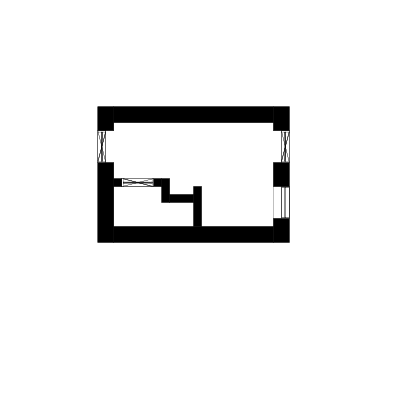
\includegraphics[width=0.505\columnwidth]{fig/scenario1_story_plan.jpg}
  \caption{Gebäudeplan des 3D Modells.}
  \label{fig:scenarios:Scenario1 Gebaeudeplan}
\end{figure}

\subsection*{Beschreibung}
Zu sehen ist der Plan eines einfachen Hauses mit einem Stockwerk.
Dieses besitzt eine Eingangstür, eine Terassentür neben einem Fenster und eine Tür, die das Badezimmer vom Hauptraum trennt.
Türen und Fenster stellen eine Herausforderung für den Planungsalgorithmus dar, da der Verlauf einer ansonsten durchgängigen Wand dadurch unterbrochen wird und Lücken aufweist.
Es gibt breite Außen- und dünne Innenwände.
Dafür müssen zwei Wandtypen definiert werden, die jeweils unterschiedliche Wanddicken vorgeben.
Diese entsprechen in ihren Maßen dem Raster, welches das \textit{LEGO System} vorgibt.
Breite Wände sollen zwei Noppen breit sein.
Daher hat deren Grundmodul Maße von 31.8$\times$15.8$\times$9.6 Millimetern mit einem Raster von 8$\times$8$\times$9.6 Millimetern.
Für die dünneren Innenwände soll eine Breite von einer Noppe verwendet werden.
Dies entspricht einem Grundmodul mit den Maßen 15.8$\times$7.8$\times$9.6 Millimetern mit einem gleichbleibenden Raster.
\begin{figure}[!ht]
  \centering
  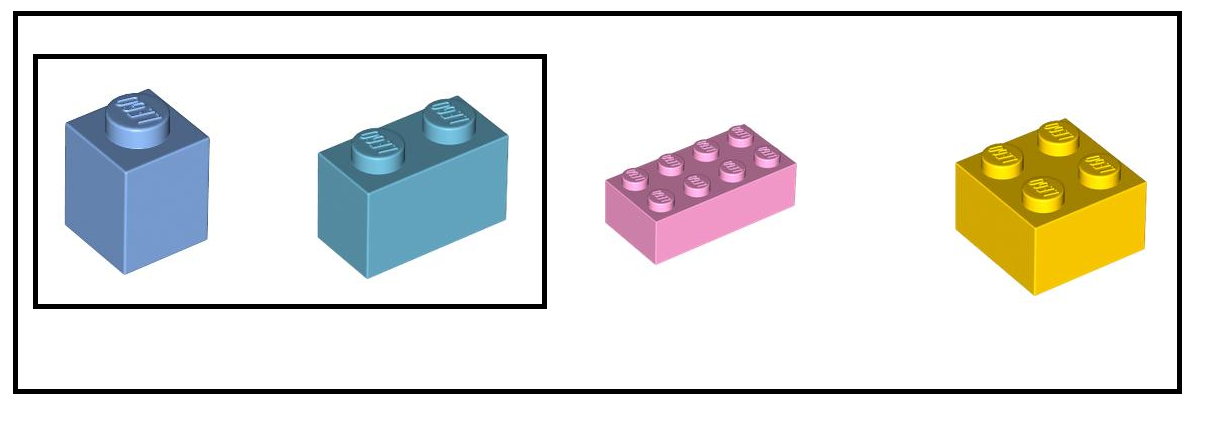
\includegraphics[width=0.6\columnwidth]{fig/scenario1_lego_set.png}
  \caption{LEGO Steintypen für die Innen- und Außenwände. (TODO Bild ist sehr hässlich)}
  \label{fig:Scenario1 Lego Set}
\end{figure}
Nicht nur die Abmessungen der Wände müssen in ein Raster fallen, auch deren Rotation wird in diesem Szenario auf 90\textdegree{} Schritte limitiert. 
Das stellt in diesem Fall eine vertretbare Enschränkung dar, da es ohnehin dem intuitiven Umgang mit LEGO Steinen und gleichzeitig dem Baustil der meisten einfachen Gebäuden entspricht.

\subsection*{Problemstellungen}
\begin{itemize}
  \item Wie können Öffnungen berücksichtigt werden?
  \item Stürze
  \item Verschiedene Wanddicken
  \item Übergänge zwischen verschiedenen Wanddicken
  \item T-Kreuzungen? Doch noch einbauen? Vlt die untere dünne wand dick machen?
\end{itemize}

\section{Scenario 3}\label{scenarios:scenario3}
Bauplandeduktion eines Gebäudemodells des KIT
\subsection*{Beschreibung}
Um das Konzept nicht nur an eigens modellierten Gebäuden zu evaluieren, werden zusätzlich externe Modelle herangezogen.
Dabei kann sich zum Beispiel an den Beispielprojekten des KIT bedient werden~\cite{KITSAMPLEHOUSE:online}.
TODO Bild von kleinem Hause
TODO überlegen ob eines der beiden riesendinger auch mal ran soll?
\subsection*{Problemstellungen}

\section{Scenario 4}\label{scenarios:scenario4}
Definition von Regelsets.
\subsection*{Beschreibung}
\subsection*{Problemstellungen}
\begin{itemize}
  \item Wie können Regelsets ohne Code vorgegeben werden? Also in welchem Format.
  \item In welcher Weise werden die Regeln dann angewendet etc?
\end{itemize}